\documentclass[12pt,letterpaper]{article}
\usepackage{graphicx,textcomp}
\usepackage{natbib}
\usepackage{setspace}
\usepackage{fullpage}
\usepackage{color}
\usepackage[reqno]{amsmath}
\usepackage{amsthm}
\usepackage{fancyvrb}
\usepackage{amssymb,enumerate}
\usepackage[all]{xy}
\usepackage{endnotes}
\usepackage{lscape}
\newtheorem{com}{Comment}
\usepackage{float}
\usepackage{hyperref}
\newtheorem{lem} {Lemma}
\newtheorem{prop}{Proposition}
\newtheorem{thm}{Theorem}
\newtheorem{defn}{Definition}
\newtheorem{cor}{Corollary}
\newtheorem{obs}{Observation}
\usepackage[compact]{titlesec}
\usepackage{dcolumn}
\usepackage{tikz}
\usetikzlibrary{arrows}
\usepackage{multirow}
\usepackage{xcolor}
\newcolumntype{.}{D{.}{.}{-1}}
\newcolumntype{d}[1]{D{.}{.}{#1}}
\definecolor{light-gray}{gray}{0.65}
\usepackage{url}
\usepackage{listings}
\usepackage{color}

\definecolor{codegreen}{rgb}{0,0.6,0}
\definecolor{codegray}{rgb}{0.5,0.5,0.5}
\definecolor{codepurple}{rgb}{0.58,0,0.82}
\definecolor{backcolour}{rgb}{0.95,0.95,0.92}

\lstdefinestyle{mystyle}{
	backgroundcolor=\color{backcolour},   
	commentstyle=\color{codegreen},
	keywordstyle=\color{magenta},
	numberstyle=\tiny\color{codegray},
	stringstyle=\color{codepurple},
	basicstyle=\footnotesize,
	breakatwhitespace=false,         
	breaklines=true,                 
	captionpos=b,                    
	keepspaces=true,                 
	numbers=left,                    
	numbersep=5pt,                  
	showspaces=false,                
	showstringspaces=false,
	showtabs=false,                  
	tabsize=2
}
\lstset{style=mystyle}
\newcommand{\Sref}[1]{Section~\ref{#1}}
\newtheorem{hyp}{Hypothesis}

\title{Problem Set 1}
\date{Han Li}
\author{Applied Stats/Quant Methods 1}

\begin{document}
	\maketitle
	
	\section*{Instructions}
	\begin{itemize}
	\item Please show your work! You may lose points by simply writing in the answer. If the problem requires you to execute commands in \texttt{R}, please include the code you used to get your answers. Please also include the \texttt{.R} file that contains your code. If you are not sure if work needs to be shown for a particular problem, please ask.
\item Your homework should be submitted electronically on GitHub.
\item This problem set is due before 23:59 on Sunday October 1, 2023. No late assignments will be accepted.
\item Total available points for this homework is 80.
	\end{itemize}
	
	\vspace{1cm}
	\section*{Question 1 (40 points): Education}

A school counselor was curious about the average of IQ of the students in her school and took a random sample of 25 students' IQ scores. The following is the data set:\\
\vspace{.5cm}

\lstinputlisting[language=R, firstline=36, lastline=36]{PS01_answersHanLi.R}  

\vspace{1cm}

\begin{enumerate}
	\item Find a 90\% confidence interval for the average student IQ in the school.\\
	\lstinputlisting[language=R, firstline=36, lastline=37]{PS01_answersHanLi.R}  
	
	\begin{verbatim}
	One Sample t-test
	data:  y
	t = 37.593, df = 24, p-value < 2.2e-16
	alternative hypothesis: true mean is not equal to 0
	90 percent confidence interval:  93.95993 102.92007
	sample estimates:
	mean of x     98.44 	
	
	To sanity check, we can also do the calculate the CI from mean:

	\end{verbatim}
	\lstinputlisting[language=R, firstline=38, lastline=40]{PS01_answersHanLi.R}  
	\begin{verbatim}
	cat(lower_90_t, upper_90_t)
	93.95993 102.9201
	\end{verbatim}
	\vspace{.5cm}
	
	
	\item Next, the school counselor was curious  whether  the average student IQ in her school is higher than the average IQ score (100) among all the schools in the country.\\ 

	\noindent Using the same sample, conduct the appropriate hypothesis test with $\alpha=0.05$.
	
		\lstinputlisting[language=R, firstline=42, lastline=44]{PS01_answersHanLi.R}  
	\begin{verbatim}
		One Sample t-test
		data:  yt = -0.59574, df = 24, 
		p-value = 0.7215
		alternative hypothesis: true mean is greater than 100
		95 percent confidence interval: 93.95993      Inf
		sample estimates:mean of x     98.44 
	\end{verbatim}
	\noindent As the p-value is 0.72, way greater than the alpha value, we have more evidence in favor of the null hypothesis, which is the IQ of the school is not higher than the average of 100. 

\end{enumerate}

\newpage

	\section*{Question 2 (40 points): Political Economy}

\noindent Researchers are curious about what affects the amount of money communities spend on addressing homelessness. The following variables constitute our data set about social welfare expenditures in the USA. \\
\vspace{.5cm}


\begin{tabular}{r|l}
	\texttt{State} &\emph{50 states in US} \\
	\texttt{Y} & \emph{per capita expenditure on shelters/housing assistance in state}\\
	\texttt{X1} &\emph{per capita personal income in state} \\
	\texttt{X2} &  \emph{Number of residents per 100,000 that are "financially insecure" in state}\\
	\texttt{X3} &  \emph{Number of people per thousand residing in urban areas in state} \\
	\texttt{Region} &  \emph{1=Northeast, 2= North Central, 3= South, 4=West} \\
\end{tabular}

\vspace{.5cm}
\noindent Explore the \texttt{expenditure} data set and import data into \texttt{R}.
\vspace{.5cm}

\begin{itemize}

\item
Please plot the relationships among \emph{Y}, \emph{X1}, \emph{X2}, and \emph{X3}? What are the correlations among them (you just need to describe the graph and the relationships among them)?

\begin{figure}[h!]\centering
	\lstinputlisting[language=R, firstline=50, lastline=52]{PS01_answersHanLi.R}
	\caption{\footnotesize Scatter plot mattix Y, X1, X2,X3}
	\label{fig:plot_1}
	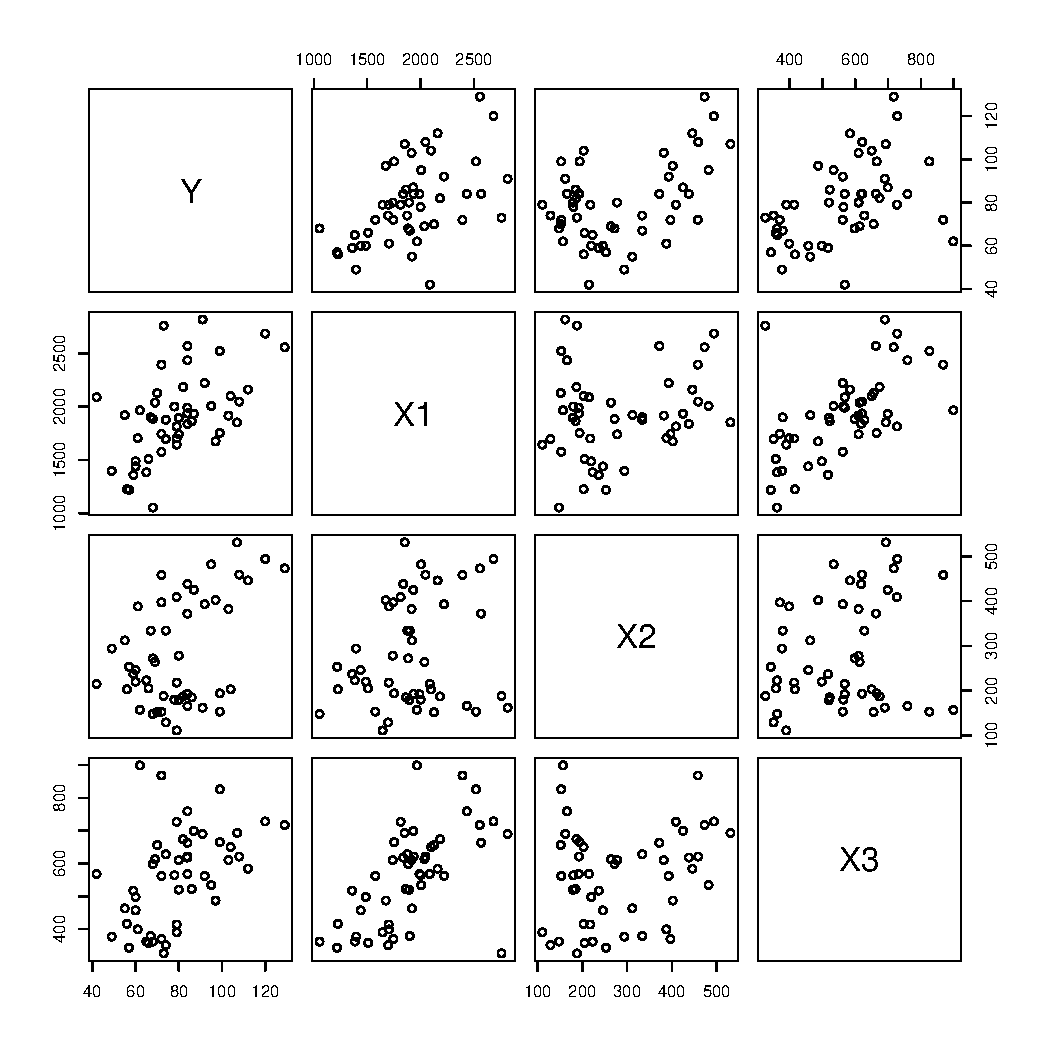
\includegraphics[width=.75\textwidth]{relationships.pdf}
\\There is a visually linear positve correlation between Y and X1, with seemingly increased variance as X1 increase.
\\There is a visually linear strong positve correlation between Y and X2.
\\There is a visually weak linear positve correlation between Y and X3.
\\There is a visually strong linear positve correlation between X1 and X2
\\There is unclear (no correlation ) or weak positive correlation between X2 and X3 visually, more analysis is needed to decide whether correlation exists.
\\There is a visually strong linear positve relationship between X1 and X3, with some outliers.
\end{figure}
\vspace{.5cm}
\item
Please plot the relationship between \emph{Y} and \emph{Region}? On average, which region has the highest per capita expenditure on housing assistance?
\vspace{.5cm}
\begin{figure}[h!]\centering
	\lstinputlisting[language=R, firstline=53, lastline=55]{PS01_answersHanLi.R}
	\caption{\footnotesize Expenditure by Region}
	\label{fig:plot_2}
	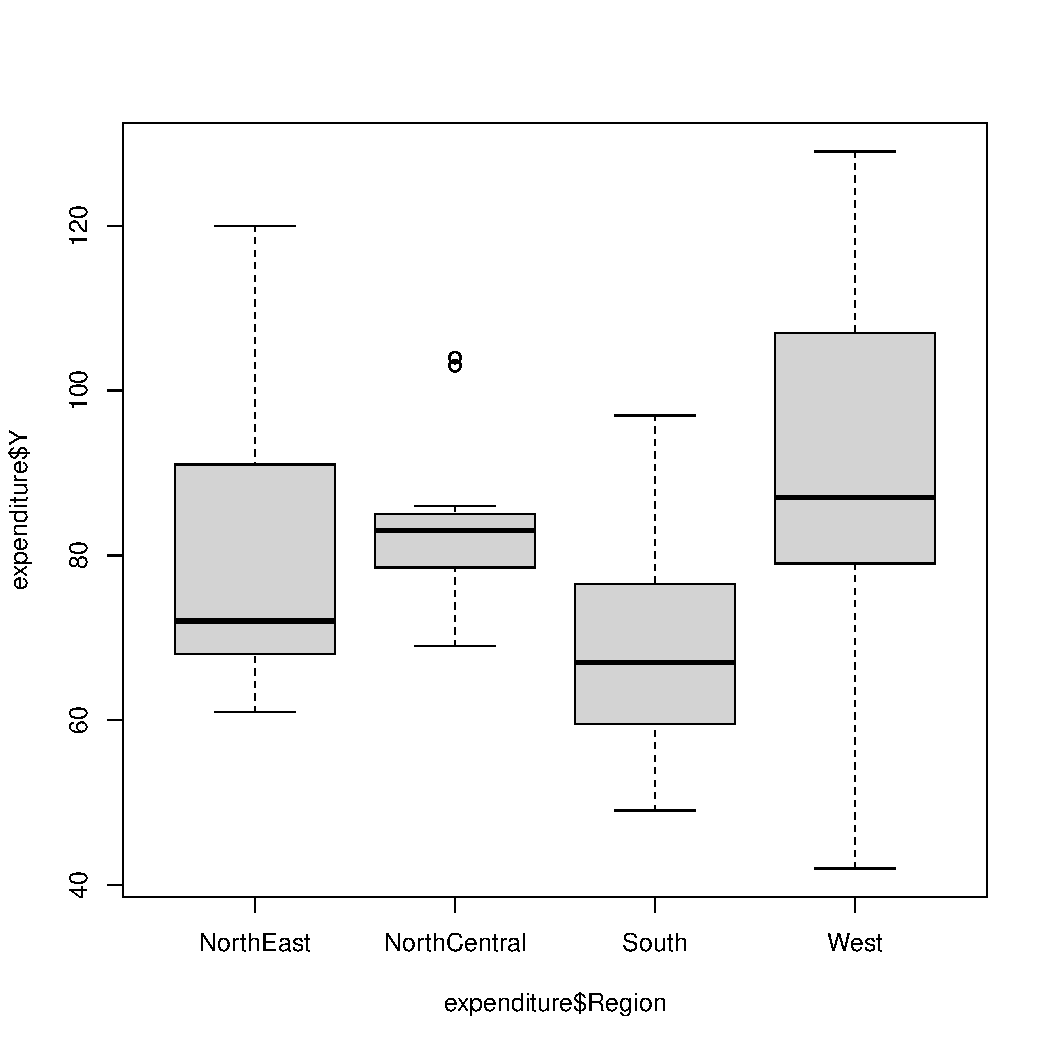
\includegraphics[width=.75\textwidth]{ExpenditurebyRegion.pdf}
\\On average the West region has the highest per capita expenditure.
\end{figure}
\item
Please plot the relationship between \emph{Y} and \emph{X1}? Describe this graph and the relationship. Reproduce the above graph including one more variable \emph{Region} and display different regions with different types of symbols and colors.
\end{itemize}

\begin{figure}[h!]\centering
	\lstinputlisting[language=R, firstline=56, lastline=58]{PS01_answersHanLi.R}
	\caption{\footnotesize Scatter plot Y and X1 }
	\label{fig:plot_3}
	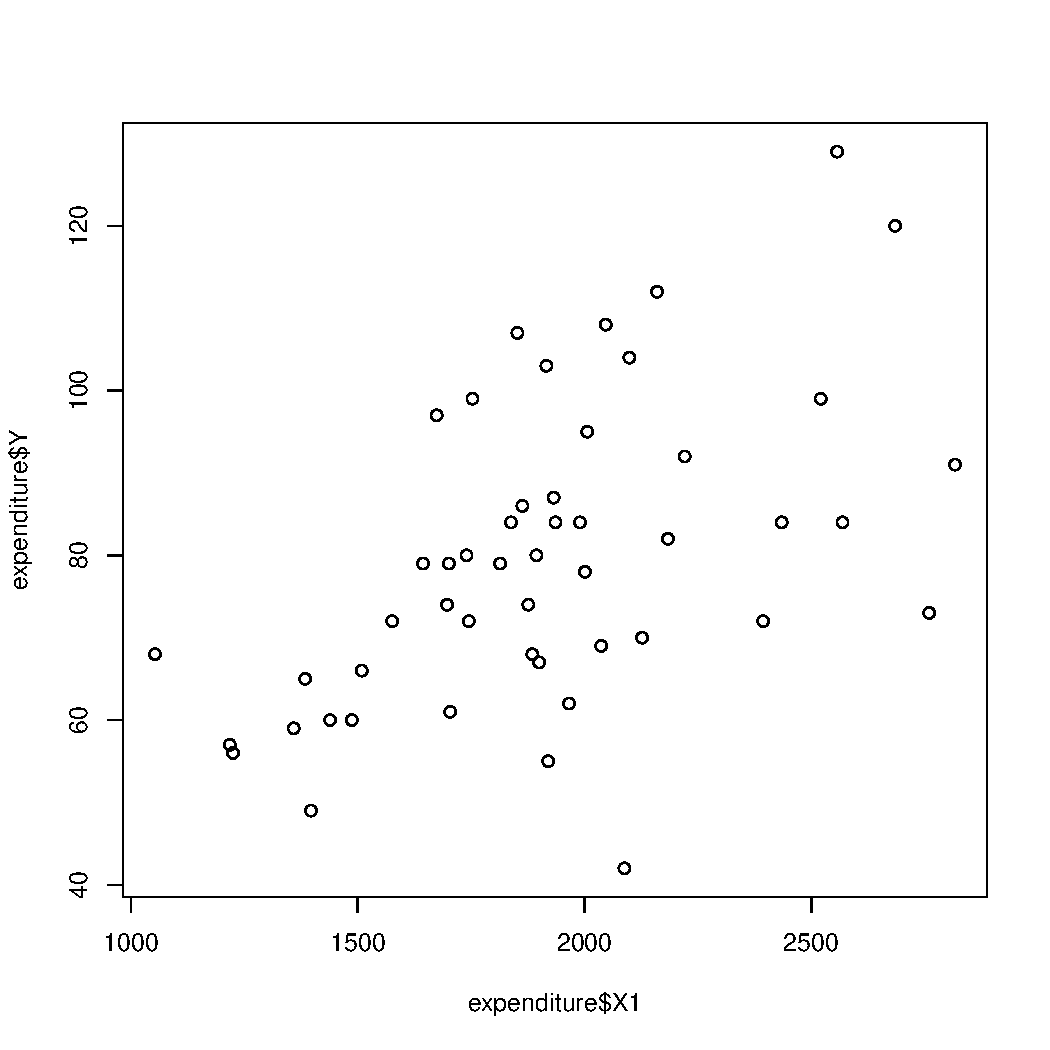
\includegraphics[width=.75\textwidth]{plotyx1.pdf}
	\\There is a positive linearcorrelation between X1,per capita personal income in state and Y, the per capita expenditure. When X1 increases, Y also increases.
\end{figure}

\begin{figure}[h!]\centering
	\lstinputlisting[language=R, firstline=59, lastline=65]{PS01_answersHanLi.R}
	\caption{\footnotesize Scatter plot Y and X1 by Region}
	\label{fig:plot_4}
	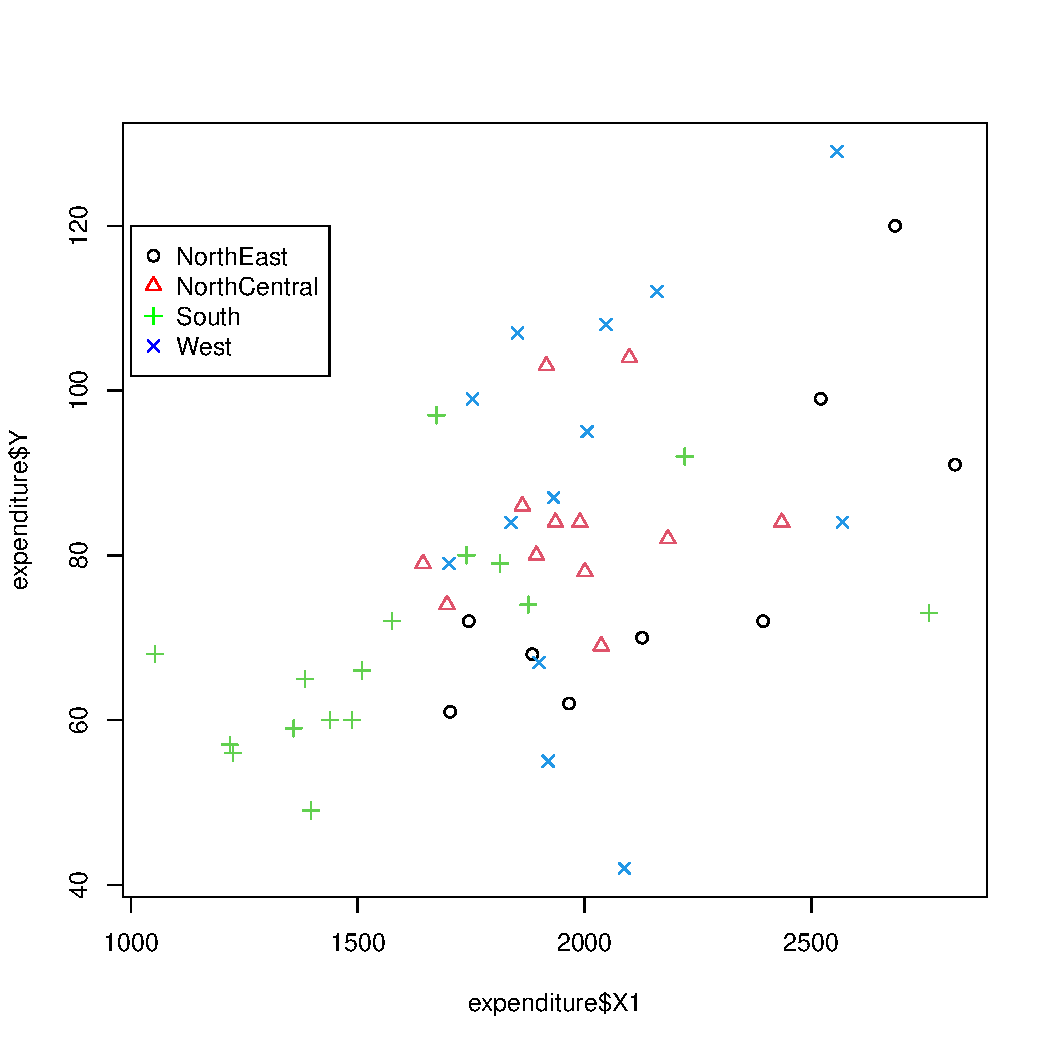
\includegraphics[width=.75\textwidth]{YbyX1Region.pdf}

\end{figure}
\end{document}
